\begin{figure}[H] \centering % Created by tikzDevice version 0.12.4 on 2023-07-24 17:06:32
% !TEX encoding = UTF-8 Unicode
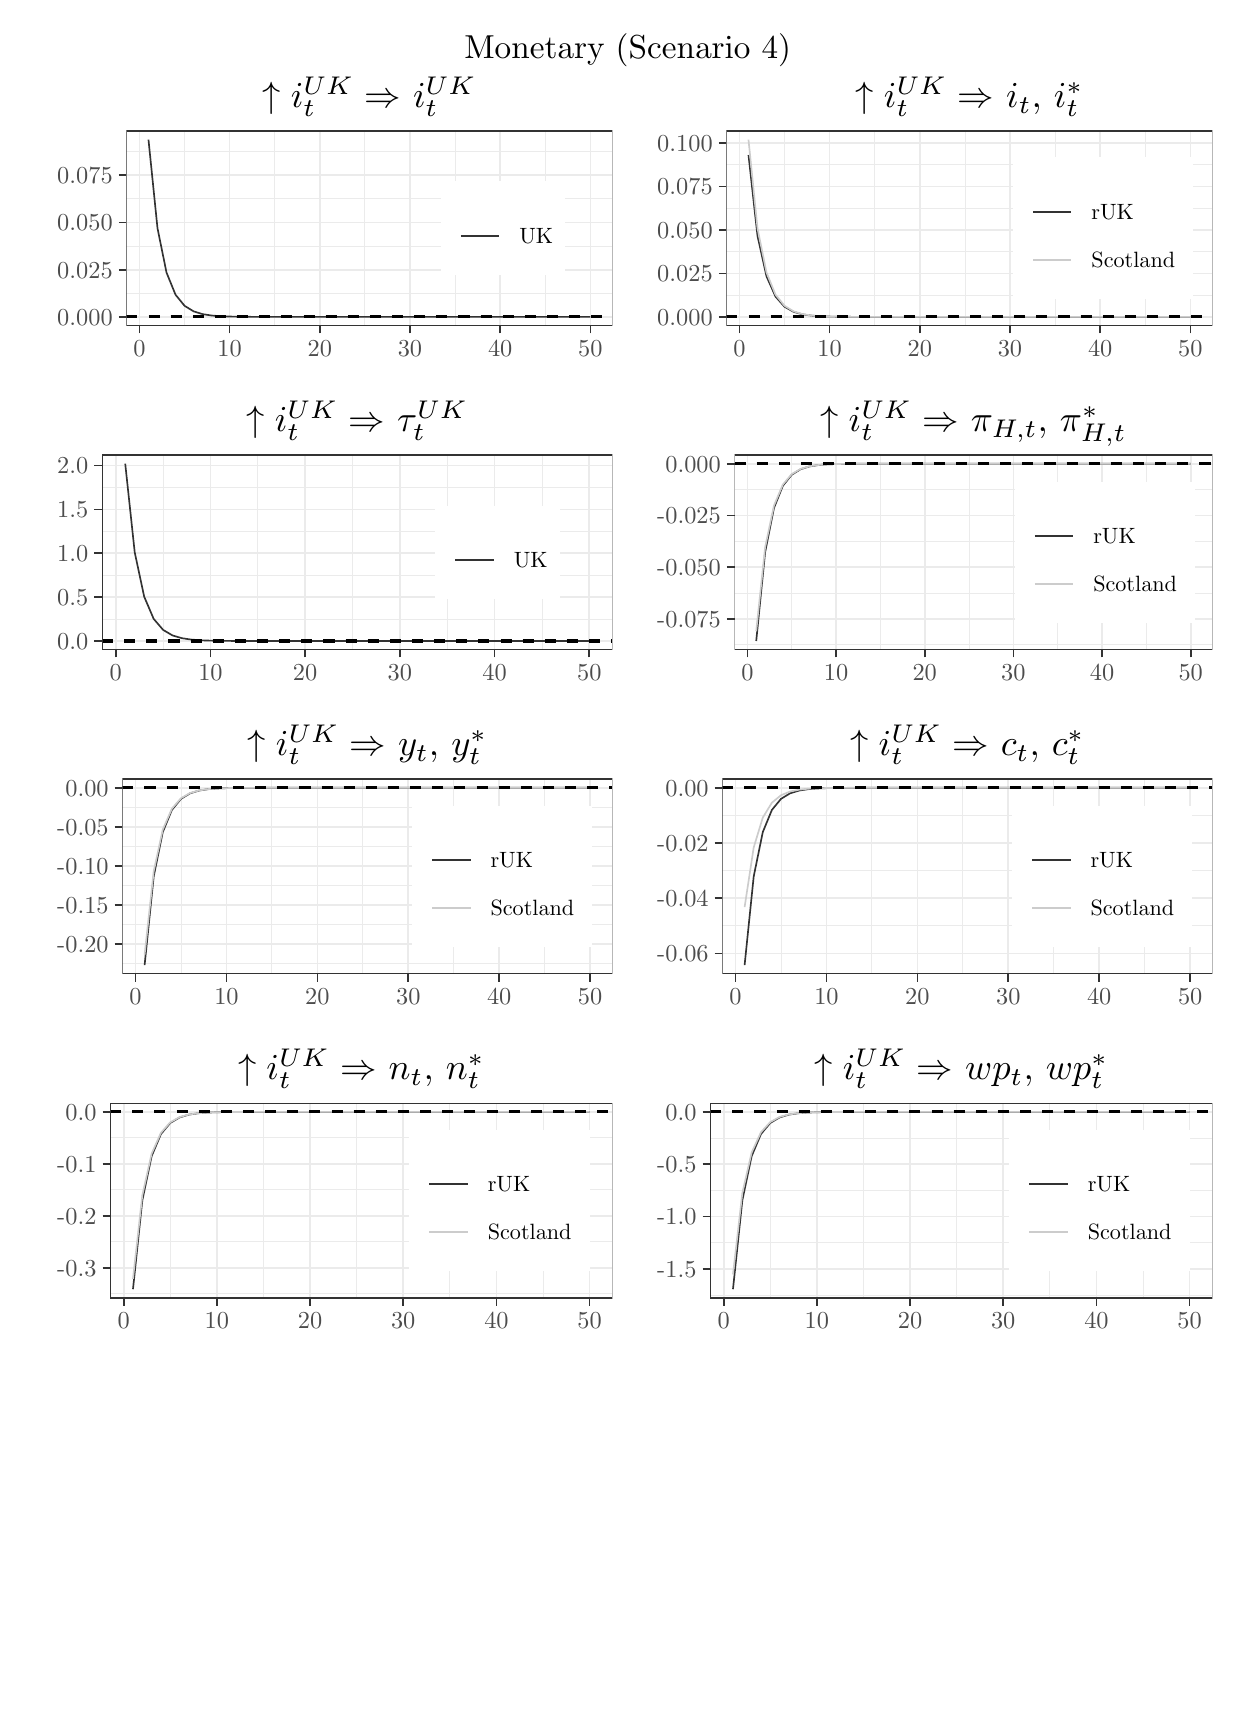
\begin{tikzpicture}[x=1pt,y=1pt]
\definecolor{fillColor}{RGB}{255,255,255}
\path[use as bounding box,fill=fillColor,fill opacity=0.00] (0,0) rectangle (433.62,599.84);
\begin{scope}
\path[clip] (  0.00,468.44) rectangle (216.81,585.55);
\definecolor{drawColor}{RGB}{255,255,255}
\definecolor{fillColor}{RGB}{255,255,255}

\path[draw=drawColor,line width= 0.6pt,line join=round,line cap=round,fill=fillColor] (  0.00,468.44) rectangle (216.81,585.55);
\end{scope}
\begin{scope}
\path[clip] ( 35.67,492.12) rectangle (211.31,562.59);
\definecolor{fillColor}{RGB}{255,255,255}

\path[fill=fillColor] ( 35.67,492.12) rectangle (211.31,562.59);
\definecolor{drawColor}{gray}{0.92}

\path[draw=drawColor,line width= 0.3pt,line join=round] ( 35.67,503.85) --
	(211.31,503.85);

\path[draw=drawColor,line width= 0.3pt,line join=round] ( 35.67,520.91) --
	(211.31,520.91);

\path[draw=drawColor,line width= 0.3pt,line join=round] ( 35.67,537.96) --
	(211.31,537.96);

\path[draw=drawColor,line width= 0.3pt,line join=round] ( 35.67,555.02) --
	(211.31,555.02);

\path[draw=drawColor,line width= 0.3pt,line join=round] ( 56.69,492.12) --
	( 56.69,562.59);

\path[draw=drawColor,line width= 0.3pt,line join=round] ( 89.27,492.12) --
	( 89.27,562.59);

\path[draw=drawColor,line width= 0.3pt,line join=round] (121.86,492.12) --
	(121.86,562.59);

\path[draw=drawColor,line width= 0.3pt,line join=round] (154.45,492.12) --
	(154.45,562.59);

\path[draw=drawColor,line width= 0.3pt,line join=round] (187.03,492.12) --
	(187.03,562.59);

\path[draw=drawColor,line width= 0.6pt,line join=round] ( 35.67,495.32) --
	(211.31,495.32);

\path[draw=drawColor,line width= 0.6pt,line join=round] ( 35.67,512.38) --
	(211.31,512.38);

\path[draw=drawColor,line width= 0.6pt,line join=round] ( 35.67,529.44) --
	(211.31,529.44);

\path[draw=drawColor,line width= 0.6pt,line join=round] ( 35.67,546.49) --
	(211.31,546.49);

\path[draw=drawColor,line width= 0.6pt,line join=round] ( 40.39,492.12) --
	( 40.39,562.59);

\path[draw=drawColor,line width= 0.6pt,line join=round] ( 72.98,492.12) --
	( 72.98,562.59);

\path[draw=drawColor,line width= 0.6pt,line join=round] (105.57,492.12) --
	(105.57,562.59);

\path[draw=drawColor,line width= 0.6pt,line join=round] (138.15,492.12) --
	(138.15,562.59);

\path[draw=drawColor,line width= 0.6pt,line join=round] (170.74,492.12) --
	(170.74,562.59);

\path[draw=drawColor,line width= 0.6pt,line join=round] (203.33,492.12) --
	(203.33,562.59);
\definecolor{drawColor}{gray}{0.20}

\path[draw=drawColor,line width= 0.6pt,line join=round] ( 43.65,559.39) --
	( 46.91,527.36) --
	( 50.17,511.34) --
	( 53.43,503.33) --
	( 56.69,499.33) --
	( 59.95,497.33) --
	( 63.20,496.32) --
	( 66.46,495.82) --
	( 69.72,495.57) --
	( 72.98,495.45) --
	( 76.24,495.39) --
	( 79.50,495.35) --
	( 82.76,495.34) --
	( 86.01,495.33) --
	( 89.27,495.33) --
	( 92.53,495.33) --
	( 95.79,495.32) --
	( 99.05,495.32) --
	(102.31,495.32) --
	(105.57,495.32) --
	(108.83,495.32) --
	(112.08,495.32) --
	(115.34,495.32) --
	(118.60,495.32) --
	(121.86,495.32) --
	(125.12,495.32) --
	(128.38,495.32) --
	(131.64,495.32) --
	(134.89,495.32) --
	(138.15,495.32) --
	(141.41,495.32) --
	(144.67,495.32) --
	(147.93,495.32) --
	(151.19,495.32) --
	(154.45,495.32) --
	(157.71,495.32) --
	(160.96,495.32) --
	(164.22,495.32) --
	(167.48,495.32) --
	(170.74,495.32) --
	(174.00,495.32) --
	(177.26,495.32) --
	(180.52,495.32) --
	(183.77,495.32) --
	(187.03,495.32) --
	(190.29,495.32) --
	(193.55,495.32) --
	(196.81,495.32) --
	(200.07,495.32) --
	(203.33,495.32);
\definecolor{drawColor}{RGB}{0,0,0}

\path[draw=drawColor,line width= 1.1pt,dash pattern=on 4pt off 4pt ,line join=round] ( 35.67,495.32) -- (211.31,495.32);
\definecolor{drawColor}{gray}{0.20}

\path[draw=drawColor,line width= 0.6pt,line join=round,line cap=round] ( 35.67,492.12) rectangle (211.31,562.59);
\end{scope}
\begin{scope}
\path[clip] (  0.00,  0.00) rectangle (433.62,599.84);
\definecolor{drawColor}{gray}{0.30}

\node[text=drawColor,anchor=base east,inner sep=0pt, outer sep=0pt, scale=  0.88] at ( 30.72,492.29) {0.000};

\node[text=drawColor,anchor=base east,inner sep=0pt, outer sep=0pt, scale=  0.88] at ( 30.72,509.35) {0.025};

\node[text=drawColor,anchor=base east,inner sep=0pt, outer sep=0pt, scale=  0.88] at ( 30.72,526.40) {0.050};

\node[text=drawColor,anchor=base east,inner sep=0pt, outer sep=0pt, scale=  0.88] at ( 30.72,543.46) {0.075};
\end{scope}
\begin{scope}
\path[clip] (  0.00,  0.00) rectangle (433.62,599.84);
\definecolor{drawColor}{gray}{0.20}

\path[draw=drawColor,line width= 0.6pt,line join=round] ( 32.92,495.32) --
	( 35.67,495.32);

\path[draw=drawColor,line width= 0.6pt,line join=round] ( 32.92,512.38) --
	( 35.67,512.38);

\path[draw=drawColor,line width= 0.6pt,line join=round] ( 32.92,529.44) --
	( 35.67,529.44);

\path[draw=drawColor,line width= 0.6pt,line join=round] ( 32.92,546.49) --
	( 35.67,546.49);
\end{scope}
\begin{scope}
\path[clip] (  0.00,  0.00) rectangle (433.62,599.84);
\definecolor{drawColor}{gray}{0.20}

\path[draw=drawColor,line width= 0.6pt,line join=round] ( 40.39,489.37) --
	( 40.39,492.12);

\path[draw=drawColor,line width= 0.6pt,line join=round] ( 72.98,489.37) --
	( 72.98,492.12);

\path[draw=drawColor,line width= 0.6pt,line join=round] (105.57,489.37) --
	(105.57,492.12);

\path[draw=drawColor,line width= 0.6pt,line join=round] (138.15,489.37) --
	(138.15,492.12);

\path[draw=drawColor,line width= 0.6pt,line join=round] (170.74,489.37) --
	(170.74,492.12);

\path[draw=drawColor,line width= 0.6pt,line join=round] (203.33,489.37) --
	(203.33,492.12);
\end{scope}
\begin{scope}
\path[clip] (  0.00,  0.00) rectangle (433.62,599.84);
\definecolor{drawColor}{gray}{0.30}

\node[text=drawColor,anchor=base,inner sep=0pt, outer sep=0pt, scale=  0.88] at ( 40.39,481.11) {0};

\node[text=drawColor,anchor=base,inner sep=0pt, outer sep=0pt, scale=  0.88] at ( 72.98,481.11) {10};

\node[text=drawColor,anchor=base,inner sep=0pt, outer sep=0pt, scale=  0.88] at (105.57,481.11) {20};

\node[text=drawColor,anchor=base,inner sep=0pt, outer sep=0pt, scale=  0.88] at (138.15,481.11) {30};

\node[text=drawColor,anchor=base,inner sep=0pt, outer sep=0pt, scale=  0.88] at (170.74,481.11) {40};

\node[text=drawColor,anchor=base,inner sep=0pt, outer sep=0pt, scale=  0.88] at (203.33,481.11) {50};
\end{scope}
\begin{scope}
\path[clip] (  0.00,  0.00) rectangle (433.62,599.84);
\definecolor{fillColor}{RGB}{255,255,255}

\path[fill=fillColor] (149.29,510.43) rectangle (194.29,544.28);
\end{scope}
\begin{scope}
\path[clip] (  0.00,  0.00) rectangle (433.62,599.84);
\definecolor{fillColor}{RGB}{255,255,255}

\path[fill=fillColor] (154.79,515.93) rectangle (172.14,533.28);
\end{scope}
\begin{scope}
\path[clip] (  0.00,  0.00) rectangle (433.62,599.84);
\definecolor{drawColor}{gray}{0.20}

\path[draw=drawColor,line width= 0.6pt,line join=round] (156.53,524.61) -- (170.40,524.61);
\end{scope}
\begin{scope}
\path[clip] (  0.00,  0.00) rectangle (433.62,599.84);
\definecolor{drawColor}{RGB}{0,0,0}

\node[text=drawColor,anchor=base west,inner sep=0pt, outer sep=0pt, scale=  0.80] at (177.64,521.85) {UK};
\end{scope}
\begin{scope}
\path[clip] (  0.00,  0.00) rectangle (433.62,599.84);
\definecolor{drawColor}{RGB}{0,0,0}

\node[text=drawColor,anchor=base,inner sep=0pt, outer sep=0pt, scale=  1.32] at (123.49,570.96) {$\uparrow  i^{UK}_t \Rightarrow $ ${i^{UK}_t}$};
\end{scope}
\begin{scope}
\path[clip] (216.81,468.44) rectangle (433.62,585.55);
\definecolor{drawColor}{RGB}{255,255,255}
\definecolor{fillColor}{RGB}{255,255,255}

\path[draw=drawColor,line width= 0.6pt,line join=round,line cap=round,fill=fillColor] (216.81,468.44) rectangle (433.62,585.55);
\end{scope}
\begin{scope}
\path[clip] (252.48,492.12) rectangle (428.12,562.59);
\definecolor{fillColor}{RGB}{255,255,255}

\path[fill=fillColor] (252.48,492.12) rectangle (428.12,562.59);
\definecolor{drawColor}{gray}{0.92}

\path[draw=drawColor,line width= 0.3pt,line join=round] (252.48,503.17) --
	(428.12,503.17);

\path[draw=drawColor,line width= 0.3pt,line join=round] (252.48,518.87) --
	(428.12,518.87);

\path[draw=drawColor,line width= 0.3pt,line join=round] (252.48,534.58) --
	(428.12,534.58);

\path[draw=drawColor,line width= 0.3pt,line join=round] (252.48,550.28) --
	(428.12,550.28);

\path[draw=drawColor,line width= 0.3pt,line join=round] (273.50,492.12) --
	(273.50,562.59);

\path[draw=drawColor,line width= 0.3pt,line join=round] (306.08,492.12) --
	(306.08,562.59);

\path[draw=drawColor,line width= 0.3pt,line join=round] (338.67,492.12) --
	(338.67,562.59);

\path[draw=drawColor,line width= 0.3pt,line join=round] (371.26,492.12) --
	(371.26,562.59);

\path[draw=drawColor,line width= 0.3pt,line join=round] (403.84,492.12) --
	(403.84,562.59);

\path[draw=drawColor,line width= 0.6pt,line join=round] (252.48,495.32) --
	(428.12,495.32);

\path[draw=drawColor,line width= 0.6pt,line join=round] (252.48,511.02) --
	(428.12,511.02);

\path[draw=drawColor,line width= 0.6pt,line join=round] (252.48,526.73) --
	(428.12,526.73);

\path[draw=drawColor,line width= 0.6pt,line join=round] (252.48,542.43) --
	(428.12,542.43);

\path[draw=drawColor,line width= 0.6pt,line join=round] (252.48,558.13) --
	(428.12,558.13);

\path[draw=drawColor,line width= 0.6pt,line join=round] (257.20,492.12) --
	(257.20,562.59);

\path[draw=drawColor,line width= 0.6pt,line join=round] (289.79,492.12) --
	(289.79,562.59);

\path[draw=drawColor,line width= 0.6pt,line join=round] (322.38,492.12) --
	(322.38,562.59);

\path[draw=drawColor,line width= 0.6pt,line join=round] (354.96,492.12) --
	(354.96,562.59);

\path[draw=drawColor,line width= 0.6pt,line join=round] (387.55,492.12) --
	(387.55,562.59);

\path[draw=drawColor,line width= 0.6pt,line join=round] (420.14,492.12) --
	(420.14,562.59);
\definecolor{drawColor}{gray}{0.20}

\path[draw=drawColor,line width= 0.6pt,line join=round] (260.46,553.82) --
	(263.72,524.57) --
	(266.98,509.95) --
	(270.24,502.64) --
	(273.50,498.98) --
	(276.76,497.15) --
	(280.01,496.24) --
	(283.27,495.78) --
	(286.53,495.55) --
	(289.79,495.44) --
	(293.05,495.38) --
	(296.31,495.35) --
	(299.57,495.34) --
	(302.82,495.33) --
	(306.08,495.33) --
	(309.34,495.33) --
	(312.60,495.32) --
	(315.86,495.32) --
	(319.12,495.32) --
	(322.38,495.32) --
	(325.64,495.32) --
	(328.89,495.32) --
	(332.15,495.32) --
	(335.41,495.32) --
	(338.67,495.32) --
	(341.93,495.32) --
	(345.19,495.32) --
	(348.45,495.32) --
	(351.70,495.32) --
	(354.96,495.32) --
	(358.22,495.32) --
	(361.48,495.32) --
	(364.74,495.32) --
	(368.00,495.32) --
	(371.26,495.32) --
	(374.52,495.32) --
	(377.77,495.32) --
	(381.03,495.32) --
	(384.29,495.32) --
	(387.55,495.32) --
	(390.81,495.32) --
	(394.07,495.32) --
	(397.33,495.32) --
	(400.58,495.32) --
	(403.84,495.32) --
	(407.10,495.32) --
	(410.36,495.32) --
	(413.62,495.32) --
	(416.88,495.32) --
	(420.14,495.32);
\definecolor{drawColor}{gray}{0.80}

\path[draw=drawColor,line width= 0.6pt,line join=round] (260.46,559.39) --
	(263.72,527.35) --
	(266.98,511.34) --
	(270.24,503.33) --
	(273.50,499.33) --
	(276.76,497.33) --
	(280.01,496.32) --
	(283.27,495.82) --
	(286.53,495.57) --
	(289.79,495.45) --
	(293.05,495.39) --
	(296.31,495.35) --
	(299.57,495.34) --
	(302.82,495.33) --
	(306.08,495.33) --
	(309.34,495.33) --
	(312.60,495.32) --
	(315.86,495.32) --
	(319.12,495.32) --
	(322.38,495.32) --
	(325.64,495.32) --
	(328.89,495.32) --
	(332.15,495.32) --
	(335.41,495.32) --
	(338.67,495.32) --
	(341.93,495.32) --
	(345.19,495.32) --
	(348.45,495.32) --
	(351.70,495.32) --
	(354.96,495.32) --
	(358.22,495.32) --
	(361.48,495.32) --
	(364.74,495.32) --
	(368.00,495.32) --
	(371.26,495.32) --
	(374.52,495.32) --
	(377.77,495.32) --
	(381.03,495.32) --
	(384.29,495.32) --
	(387.55,495.32) --
	(390.81,495.32) --
	(394.07,495.32) --
	(397.33,495.32) --
	(400.58,495.32) --
	(403.84,495.32) --
	(407.10,495.32) --
	(410.36,495.32) --
	(413.62,495.32) --
	(416.88,495.32) --
	(420.14,495.32);
\definecolor{drawColor}{RGB}{0,0,0}

\path[draw=drawColor,line width= 1.1pt,dash pattern=on 4pt off 4pt ,line join=round] (252.48,495.32) -- (428.12,495.32);
\definecolor{drawColor}{gray}{0.20}

\path[draw=drawColor,line width= 0.6pt,line join=round,line cap=round] (252.48,492.12) rectangle (428.12,562.59);
\end{scope}
\begin{scope}
\path[clip] (  0.00,  0.00) rectangle (433.62,599.84);
\definecolor{drawColor}{gray}{0.30}

\node[text=drawColor,anchor=base east,inner sep=0pt, outer sep=0pt, scale=  0.88] at (247.53,492.29) {0.000};

\node[text=drawColor,anchor=base east,inner sep=0pt, outer sep=0pt, scale=  0.88] at (247.53,507.99) {0.025};

\node[text=drawColor,anchor=base east,inner sep=0pt, outer sep=0pt, scale=  0.88] at (247.53,523.69) {0.050};

\node[text=drawColor,anchor=base east,inner sep=0pt, outer sep=0pt, scale=  0.88] at (247.53,539.40) {0.075};

\node[text=drawColor,anchor=base east,inner sep=0pt, outer sep=0pt, scale=  0.88] at (247.53,555.10) {0.100};
\end{scope}
\begin{scope}
\path[clip] (  0.00,  0.00) rectangle (433.62,599.84);
\definecolor{drawColor}{gray}{0.20}

\path[draw=drawColor,line width= 0.6pt,line join=round] (249.73,495.32) --
	(252.48,495.32);

\path[draw=drawColor,line width= 0.6pt,line join=round] (249.73,511.02) --
	(252.48,511.02);

\path[draw=drawColor,line width= 0.6pt,line join=round] (249.73,526.73) --
	(252.48,526.73);

\path[draw=drawColor,line width= 0.6pt,line join=round] (249.73,542.43) --
	(252.48,542.43);

\path[draw=drawColor,line width= 0.6pt,line join=round] (249.73,558.13) --
	(252.48,558.13);
\end{scope}
\begin{scope}
\path[clip] (  0.00,  0.00) rectangle (433.62,599.84);
\definecolor{drawColor}{gray}{0.20}

\path[draw=drawColor,line width= 0.6pt,line join=round] (257.20,489.37) --
	(257.20,492.12);

\path[draw=drawColor,line width= 0.6pt,line join=round] (289.79,489.37) --
	(289.79,492.12);

\path[draw=drawColor,line width= 0.6pt,line join=round] (322.38,489.37) --
	(322.38,492.12);

\path[draw=drawColor,line width= 0.6pt,line join=round] (354.96,489.37) --
	(354.96,492.12);

\path[draw=drawColor,line width= 0.6pt,line join=round] (387.55,489.37) --
	(387.55,492.12);

\path[draw=drawColor,line width= 0.6pt,line join=round] (420.14,489.37) --
	(420.14,492.12);
\end{scope}
\begin{scope}
\path[clip] (  0.00,  0.00) rectangle (433.62,599.84);
\definecolor{drawColor}{gray}{0.30}

\node[text=drawColor,anchor=base,inner sep=0pt, outer sep=0pt, scale=  0.88] at (257.20,481.11) {0};

\node[text=drawColor,anchor=base,inner sep=0pt, outer sep=0pt, scale=  0.88] at (289.79,481.11) {10};

\node[text=drawColor,anchor=base,inner sep=0pt, outer sep=0pt, scale=  0.88] at (322.38,481.11) {20};

\node[text=drawColor,anchor=base,inner sep=0pt, outer sep=0pt, scale=  0.88] at (354.96,481.11) {30};

\node[text=drawColor,anchor=base,inner sep=0pt, outer sep=0pt, scale=  0.88] at (387.55,481.11) {40};

\node[text=drawColor,anchor=base,inner sep=0pt, outer sep=0pt, scale=  0.88] at (420.14,481.11) {50};
\end{scope}
\begin{scope}
\path[clip] (  0.00,  0.00) rectangle (433.62,599.84);
\definecolor{fillColor}{RGB}{255,255,255}

\path[fill=fillColor] (356.06,501.76) rectangle (421.15,552.95);
\end{scope}
\begin{scope}
\path[clip] (  0.00,  0.00) rectangle (433.62,599.84);
\definecolor{fillColor}{RGB}{255,255,255}

\path[fill=fillColor] (361.56,524.61) rectangle (378.90,541.95);
\end{scope}
\begin{scope}
\path[clip] (  0.00,  0.00) rectangle (433.62,599.84);
\definecolor{drawColor}{gray}{0.20}

\path[draw=drawColor,line width= 0.6pt,line join=round] (363.29,533.28) -- (377.17,533.28);
\end{scope}
\begin{scope}
\path[clip] (  0.00,  0.00) rectangle (433.62,599.84);
\definecolor{fillColor}{RGB}{255,255,255}

\path[fill=fillColor] (361.56,507.26) rectangle (378.90,524.61);
\end{scope}
\begin{scope}
\path[clip] (  0.00,  0.00) rectangle (433.62,599.84);
\definecolor{drawColor}{gray}{0.80}

\path[draw=drawColor,line width= 0.6pt,line join=round] (363.29,515.93) -- (377.17,515.93);
\end{scope}
\begin{scope}
\path[clip] (  0.00,  0.00) rectangle (433.62,599.84);
\definecolor{drawColor}{RGB}{0,0,0}

\node[text=drawColor,anchor=base west,inner sep=0pt, outer sep=0pt, scale=  0.80] at (384.40,530.52) {rUK};
\end{scope}
\begin{scope}
\path[clip] (  0.00,  0.00) rectangle (433.62,599.84);
\definecolor{drawColor}{RGB}{0,0,0}

\node[text=drawColor,anchor=base west,inner sep=0pt, outer sep=0pt, scale=  0.80] at (384.40,513.18) {Scotland};
\end{scope}
\begin{scope}
\path[clip] (  0.00,  0.00) rectangle (433.62,599.84);
\definecolor{drawColor}{RGB}{0,0,0}

\node[text=drawColor,anchor=base,inner sep=0pt, outer sep=0pt, scale=  1.32] at (340.30,570.96) {$\uparrow  i^{UK}_t \Rightarrow $ ${i_t}$, ${i^*_t}$};
\end{scope}
\begin{scope}
\path[clip] (  0.00,351.33) rectangle (216.81,468.44);
\definecolor{drawColor}{RGB}{255,255,255}
\definecolor{fillColor}{RGB}{255,255,255}

\path[draw=drawColor,line width= 0.6pt,line join=round,line cap=round,fill=fillColor] (  0.00,351.33) rectangle (216.81,468.44);
\end{scope}
\begin{scope}
\path[clip] ( 26.87,375.01) rectangle (211.31,445.48);
\definecolor{fillColor}{RGB}{255,255,255}

\path[fill=fillColor] ( 26.87,375.01) rectangle (211.31,445.48);
\definecolor{drawColor}{gray}{0.92}

\path[draw=drawColor,line width= 0.3pt,line join=round] ( 26.87,386.14) --
	(211.31,386.14);

\path[draw=drawColor,line width= 0.3pt,line join=round] ( 26.87,401.99) --
	(211.31,401.99);

\path[draw=drawColor,line width= 0.3pt,line join=round] ( 26.87,417.84) --
	(211.31,417.84);

\path[draw=drawColor,line width= 0.3pt,line join=round] ( 26.87,433.69) --
	(211.31,433.69);

\path[draw=drawColor,line width= 0.3pt,line join=round] ( 48.94,375.01) --
	( 48.94,445.48);

\path[draw=drawColor,line width= 0.3pt,line join=round] ( 83.16,375.01) --
	( 83.16,445.48);

\path[draw=drawColor,line width= 0.3pt,line join=round] (117.38,375.01) --
	(117.38,445.48);

\path[draw=drawColor,line width= 0.3pt,line join=round] (151.60,375.01) --
	(151.60,445.48);

\path[draw=drawColor,line width= 0.3pt,line join=round] (185.82,375.01) --
	(185.82,445.48);

\path[draw=drawColor,line width= 0.6pt,line join=round] ( 26.87,378.21) --
	(211.31,378.21);

\path[draw=drawColor,line width= 0.6pt,line join=round] ( 26.87,394.06) --
	(211.31,394.06);

\path[draw=drawColor,line width= 0.6pt,line join=round] ( 26.87,409.91) --
	(211.31,409.91);

\path[draw=drawColor,line width= 0.6pt,line join=round] ( 26.87,425.76) --
	(211.31,425.76);

\path[draw=drawColor,line width= 0.6pt,line join=round] ( 26.87,441.61) --
	(211.31,441.61);

\path[draw=drawColor,line width= 0.6pt,line join=round] ( 31.83,375.01) --
	( 31.83,445.48);

\path[draw=drawColor,line width= 0.6pt,line join=round] ( 66.05,375.01) --
	( 66.05,445.48);

\path[draw=drawColor,line width= 0.6pt,line join=round] (100.27,375.01) --
	(100.27,445.48);

\path[draw=drawColor,line width= 0.6pt,line join=round] (134.49,375.01) --
	(134.49,445.48);

\path[draw=drawColor,line width= 0.6pt,line join=round] (168.71,375.01) --
	(168.71,445.48);

\path[draw=drawColor,line width= 0.6pt,line join=round] (202.93,375.01) --
	(202.93,445.48);
\definecolor{drawColor}{gray}{0.20}

\path[draw=drawColor,line width= 0.6pt,line join=round] ( 35.25,442.28) --
	( 38.68,410.25) --
	( 42.10,394.23) --
	( 45.52,386.22) --
	( 48.94,382.22) --
	( 52.36,380.21) --
	( 55.79,379.21) --
	( 59.21,378.71) --
	( 62.63,378.46) --
	( 66.05,378.34) --
	( 69.47,378.28) --
	( 72.90,378.24) --
	( 76.32,378.23) --
	( 79.74,378.22) --
	( 83.16,378.22) --
	( 86.58,378.21) --
	( 90.00,378.21) --
	( 93.43,378.21) --
	( 96.85,378.21) --
	(100.27,378.21) --
	(103.69,378.21) --
	(107.11,378.21) --
	(110.54,378.21) --
	(113.96,378.21) --
	(117.38,378.21) --
	(120.80,378.21) --
	(124.22,378.21) --
	(127.65,378.21) --
	(131.07,378.21) --
	(134.49,378.21) --
	(137.91,378.21) --
	(141.33,378.21) --
	(144.75,378.21) --
	(148.18,378.21) --
	(151.60,378.21) --
	(155.02,378.21) --
	(158.44,378.21) --
	(161.86,378.21) --
	(165.29,378.21) --
	(168.71,378.21) --
	(172.13,378.21) --
	(175.55,378.21) --
	(178.97,378.21) --
	(182.40,378.21) --
	(185.82,378.21) --
	(189.24,378.21) --
	(192.66,378.21) --
	(196.08,378.21) --
	(199.50,378.21) --
	(202.93,378.21);
\definecolor{drawColor}{RGB}{0,0,0}

\path[draw=drawColor,line width= 1.1pt,dash pattern=on 4pt off 4pt ,line join=round] ( 26.87,378.21) -- (211.31,378.21);
\definecolor{drawColor}{gray}{0.20}

\path[draw=drawColor,line width= 0.6pt,line join=round,line cap=round] ( 26.87,375.01) rectangle (211.31,445.48);
\end{scope}
\begin{scope}
\path[clip] (  0.00,  0.00) rectangle (433.62,599.84);
\definecolor{drawColor}{gray}{0.30}

\node[text=drawColor,anchor=base east,inner sep=0pt, outer sep=0pt, scale=  0.88] at ( 21.92,375.18) {0.0};

\node[text=drawColor,anchor=base east,inner sep=0pt, outer sep=0pt, scale=  0.88] at ( 21.92,391.03) {0.5};

\node[text=drawColor,anchor=base east,inner sep=0pt, outer sep=0pt, scale=  0.88] at ( 21.92,406.88) {1.0};

\node[text=drawColor,anchor=base east,inner sep=0pt, outer sep=0pt, scale=  0.88] at ( 21.92,422.73) {1.5};

\node[text=drawColor,anchor=base east,inner sep=0pt, outer sep=0pt, scale=  0.88] at ( 21.92,438.58) {2.0};
\end{scope}
\begin{scope}
\path[clip] (  0.00,  0.00) rectangle (433.62,599.84);
\definecolor{drawColor}{gray}{0.20}

\path[draw=drawColor,line width= 0.6pt,line join=round] ( 24.12,378.21) --
	( 26.87,378.21);

\path[draw=drawColor,line width= 0.6pt,line join=round] ( 24.12,394.06) --
	( 26.87,394.06);

\path[draw=drawColor,line width= 0.6pt,line join=round] ( 24.12,409.91) --
	( 26.87,409.91);

\path[draw=drawColor,line width= 0.6pt,line join=round] ( 24.12,425.76) --
	( 26.87,425.76);

\path[draw=drawColor,line width= 0.6pt,line join=round] ( 24.12,441.61) --
	( 26.87,441.61);
\end{scope}
\begin{scope}
\path[clip] (  0.00,  0.00) rectangle (433.62,599.84);
\definecolor{drawColor}{gray}{0.20}

\path[draw=drawColor,line width= 0.6pt,line join=round] ( 31.83,372.26) --
	( 31.83,375.01);

\path[draw=drawColor,line width= 0.6pt,line join=round] ( 66.05,372.26) --
	( 66.05,375.01);

\path[draw=drawColor,line width= 0.6pt,line join=round] (100.27,372.26) --
	(100.27,375.01);

\path[draw=drawColor,line width= 0.6pt,line join=round] (134.49,372.26) --
	(134.49,375.01);

\path[draw=drawColor,line width= 0.6pt,line join=round] (168.71,372.26) --
	(168.71,375.01);

\path[draw=drawColor,line width= 0.6pt,line join=round] (202.93,372.26) --
	(202.93,375.01);
\end{scope}
\begin{scope}
\path[clip] (  0.00,  0.00) rectangle (433.62,599.84);
\definecolor{drawColor}{gray}{0.30}

\node[text=drawColor,anchor=base,inner sep=0pt, outer sep=0pt, scale=  0.88] at ( 31.83,364.00) {0};

\node[text=drawColor,anchor=base,inner sep=0pt, outer sep=0pt, scale=  0.88] at ( 66.05,364.00) {10};

\node[text=drawColor,anchor=base,inner sep=0pt, outer sep=0pt, scale=  0.88] at (100.27,364.00) {20};

\node[text=drawColor,anchor=base,inner sep=0pt, outer sep=0pt, scale=  0.88] at (134.49,364.00) {30};

\node[text=drawColor,anchor=base,inner sep=0pt, outer sep=0pt, scale=  0.88] at (168.71,364.00) {40};

\node[text=drawColor,anchor=base,inner sep=0pt, outer sep=0pt, scale=  0.88] at (202.93,364.00) {50};
\end{scope}
\begin{scope}
\path[clip] (  0.00,  0.00) rectangle (433.62,599.84);
\definecolor{fillColor}{RGB}{255,255,255}

\path[fill=fillColor] (147.31,393.32) rectangle (192.31,427.17);
\end{scope}
\begin{scope}
\path[clip] (  0.00,  0.00) rectangle (433.62,599.84);
\definecolor{fillColor}{RGB}{255,255,255}

\path[fill=fillColor] (152.81,398.82) rectangle (170.16,416.17);
\end{scope}
\begin{scope}
\path[clip] (  0.00,  0.00) rectangle (433.62,599.84);
\definecolor{drawColor}{gray}{0.20}

\path[draw=drawColor,line width= 0.6pt,line join=round] (154.55,407.50) -- (168.42,407.50);
\end{scope}
\begin{scope}
\path[clip] (  0.00,  0.00) rectangle (433.62,599.84);
\definecolor{drawColor}{RGB}{0,0,0}

\node[text=drawColor,anchor=base west,inner sep=0pt, outer sep=0pt, scale=  0.80] at (175.66,404.74) {UK};
\end{scope}
\begin{scope}
\path[clip] (  0.00,  0.00) rectangle (433.62,599.84);
\definecolor{drawColor}{RGB}{0,0,0}

\node[text=drawColor,anchor=base,inner sep=0pt, outer sep=0pt, scale=  1.32] at (119.09,453.85) {$\uparrow  i^{UK}_t \Rightarrow $ ${\tau^{UK}_t}$};
\end{scope}
\begin{scope}
\path[clip] (216.81,351.33) rectangle (433.62,468.44);
\definecolor{drawColor}{RGB}{255,255,255}
\definecolor{fillColor}{RGB}{255,255,255}

\path[draw=drawColor,line width= 0.6pt,line join=round,line cap=round,fill=fillColor] (216.81,351.33) rectangle (433.62,468.44);
\end{scope}
\begin{scope}
\path[clip] (255.41,375.01) rectangle (428.12,445.48);
\definecolor{fillColor}{RGB}{255,255,255}

\path[fill=fillColor] (255.41,375.01) rectangle (428.12,445.48);
\definecolor{drawColor}{gray}{0.92}

\path[draw=drawColor,line width= 0.3pt,line join=round] (255.41,376.81) --
	(428.12,376.81);

\path[draw=drawColor,line width= 0.3pt,line join=round] (255.41,395.51) --
	(428.12,395.51);

\path[draw=drawColor,line width= 0.3pt,line join=round] (255.41,414.22) --
	(428.12,414.22);

\path[draw=drawColor,line width= 0.3pt,line join=round] (255.41,432.93) --
	(428.12,432.93);

\path[draw=drawColor,line width= 0.3pt,line join=round] (276.08,375.01) --
	(276.08,445.48);

\path[draw=drawColor,line width= 0.3pt,line join=round] (308.12,375.01) --
	(308.12,445.48);

\path[draw=drawColor,line width= 0.3pt,line join=round] (340.16,375.01) --
	(340.16,445.48);

\path[draw=drawColor,line width= 0.3pt,line join=round] (372.21,375.01) --
	(372.21,445.48);

\path[draw=drawColor,line width= 0.3pt,line join=round] (404.25,375.01) --
	(404.25,445.48);

\path[draw=drawColor,line width= 0.6pt,line join=round] (255.41,386.16) --
	(428.12,386.16);

\path[draw=drawColor,line width= 0.6pt,line join=round] (255.41,404.87) --
	(428.12,404.87);

\path[draw=drawColor,line width= 0.6pt,line join=round] (255.41,423.57) --
	(428.12,423.57);

\path[draw=drawColor,line width= 0.6pt,line join=round] (255.41,442.28) --
	(428.12,442.28);

\path[draw=drawColor,line width= 0.6pt,line join=round] (260.06,375.01) --
	(260.06,445.48);

\path[draw=drawColor,line width= 0.6pt,line join=round] (292.10,375.01) --
	(292.10,445.48);

\path[draw=drawColor,line width= 0.6pt,line join=round] (324.14,375.01) --
	(324.14,445.48);

\path[draw=drawColor,line width= 0.6pt,line join=round] (356.18,375.01) --
	(356.18,445.48);

\path[draw=drawColor,line width= 0.6pt,line join=round] (388.23,375.01) --
	(388.23,445.48);

\path[draw=drawColor,line width= 0.6pt,line join=round] (420.27,375.01) --
	(420.27,445.48);
\definecolor{drawColor}{gray}{0.20}

\path[draw=drawColor,line width= 0.6pt,line join=round] (263.26,378.21) --
	(266.47,410.25) --
	(269.67,426.26) --
	(272.87,434.27) --
	(276.08,438.27) --
	(279.28,440.28) --
	(282.49,441.28) --
	(285.69,441.78) --
	(288.90,442.03) --
	(292.10,442.15) --
	(295.30,442.22) --
	(298.51,442.25) --
	(301.71,442.26) --
	(304.92,442.27) --
	(308.12,442.27) --
	(311.33,442.28) --
	(314.53,442.28) --
	(317.73,442.28) --
	(320.94,442.28) --
	(324.14,442.28) --
	(327.35,442.28) --
	(330.55,442.28) --
	(333.76,442.28) --
	(336.96,442.28) --
	(340.16,442.28) --
	(343.37,442.28) --
	(346.57,442.28) --
	(349.78,442.28) --
	(352.98,442.28) --
	(356.18,442.28) --
	(359.39,442.28) --
	(362.59,442.28) --
	(365.80,442.28) --
	(369.00,442.28) --
	(372.21,442.28) --
	(375.41,442.28) --
	(378.61,442.28) --
	(381.82,442.28) --
	(385.02,442.28) --
	(388.23,442.28) --
	(391.43,442.28) --
	(394.64,442.28) --
	(397.84,442.28) --
	(401.04,442.28) --
	(404.25,442.28) --
	(407.45,442.28) --
	(410.66,442.28) --
	(413.86,442.28) --
	(417.07,442.28) --
	(420.27,442.28);
\definecolor{drawColor}{gray}{0.80}

\path[draw=drawColor,line width= 0.6pt,line join=round] (263.26,381.81) --
	(266.47,412.04) --
	(269.67,427.16) --
	(272.87,434.72) --
	(276.08,438.50) --
	(279.28,440.39) --
	(282.49,441.33) --
	(285.69,441.81) --
	(288.90,442.04) --
	(292.10,442.16) --
	(295.30,442.22) --
	(298.51,442.25) --
	(301.71,442.26) --
	(304.92,442.27) --
	(308.12,442.27) --
	(311.33,442.28) --
	(314.53,442.28) --
	(317.73,442.28) --
	(320.94,442.28) --
	(324.14,442.28) --
	(327.35,442.28) --
	(330.55,442.28) --
	(333.76,442.28) --
	(336.96,442.28) --
	(340.16,442.28) --
	(343.37,442.28) --
	(346.57,442.28) --
	(349.78,442.28) --
	(352.98,442.28) --
	(356.18,442.28) --
	(359.39,442.28) --
	(362.59,442.28) --
	(365.80,442.28) --
	(369.00,442.28) --
	(372.21,442.28) --
	(375.41,442.28) --
	(378.61,442.28) --
	(381.82,442.28) --
	(385.02,442.28) --
	(388.23,442.28) --
	(391.43,442.28) --
	(394.64,442.28) --
	(397.84,442.28) --
	(401.04,442.28) --
	(404.25,442.28) --
	(407.45,442.28) --
	(410.66,442.28) --
	(413.86,442.28) --
	(417.07,442.28) --
	(420.27,442.28);
\definecolor{drawColor}{RGB}{0,0,0}

\path[draw=drawColor,line width= 1.1pt,dash pattern=on 4pt off 4pt ,line join=round] (255.41,442.28) -- (428.12,442.28);
\definecolor{drawColor}{gray}{0.20}

\path[draw=drawColor,line width= 0.6pt,line join=round,line cap=round] (255.41,375.01) rectangle (428.12,445.48);
\end{scope}
\begin{scope}
\path[clip] (  0.00,  0.00) rectangle (433.62,599.84);
\definecolor{drawColor}{gray}{0.30}

\node[text=drawColor,anchor=base east,inner sep=0pt, outer sep=0pt, scale=  0.88] at (250.46,383.13) {-0.075};

\node[text=drawColor,anchor=base east,inner sep=0pt, outer sep=0pt, scale=  0.88] at (250.46,401.84) {-0.050};

\node[text=drawColor,anchor=base east,inner sep=0pt, outer sep=0pt, scale=  0.88] at (250.46,420.54) {-0.025};

\node[text=drawColor,anchor=base east,inner sep=0pt, outer sep=0pt, scale=  0.88] at (250.46,439.25) {0.000};
\end{scope}
\begin{scope}
\path[clip] (  0.00,  0.00) rectangle (433.62,599.84);
\definecolor{drawColor}{gray}{0.20}

\path[draw=drawColor,line width= 0.6pt,line join=round] (252.66,386.16) --
	(255.41,386.16);

\path[draw=drawColor,line width= 0.6pt,line join=round] (252.66,404.87) --
	(255.41,404.87);

\path[draw=drawColor,line width= 0.6pt,line join=round] (252.66,423.57) --
	(255.41,423.57);

\path[draw=drawColor,line width= 0.6pt,line join=round] (252.66,442.28) --
	(255.41,442.28);
\end{scope}
\begin{scope}
\path[clip] (  0.00,  0.00) rectangle (433.62,599.84);
\definecolor{drawColor}{gray}{0.20}

\path[draw=drawColor,line width= 0.6pt,line join=round] (260.06,372.26) --
	(260.06,375.01);

\path[draw=drawColor,line width= 0.6pt,line join=round] (292.10,372.26) --
	(292.10,375.01);

\path[draw=drawColor,line width= 0.6pt,line join=round] (324.14,372.26) --
	(324.14,375.01);

\path[draw=drawColor,line width= 0.6pt,line join=round] (356.18,372.26) --
	(356.18,375.01);

\path[draw=drawColor,line width= 0.6pt,line join=round] (388.23,372.26) --
	(388.23,375.01);

\path[draw=drawColor,line width= 0.6pt,line join=round] (420.27,372.26) --
	(420.27,375.01);
\end{scope}
\begin{scope}
\path[clip] (  0.00,  0.00) rectangle (433.62,599.84);
\definecolor{drawColor}{gray}{0.30}

\node[text=drawColor,anchor=base,inner sep=0pt, outer sep=0pt, scale=  0.88] at (260.06,364.00) {0};

\node[text=drawColor,anchor=base,inner sep=0pt, outer sep=0pt, scale=  0.88] at (292.10,364.00) {10};

\node[text=drawColor,anchor=base,inner sep=0pt, outer sep=0pt, scale=  0.88] at (324.14,364.00) {20};

\node[text=drawColor,anchor=base,inner sep=0pt, outer sep=0pt, scale=  0.88] at (356.18,364.00) {30};

\node[text=drawColor,anchor=base,inner sep=0pt, outer sep=0pt, scale=  0.88] at (388.23,364.00) {40};

\node[text=drawColor,anchor=base,inner sep=0pt, outer sep=0pt, scale=  0.88] at (420.27,364.00) {50};
\end{scope}
\begin{scope}
\path[clip] (  0.00,  0.00) rectangle (433.62,599.84);
\definecolor{fillColor}{RGB}{255,255,255}

\path[fill=fillColor] (356.72,384.65) rectangle (421.81,435.84);
\end{scope}
\begin{scope}
\path[clip] (  0.00,  0.00) rectangle (433.62,599.84);
\definecolor{fillColor}{RGB}{255,255,255}

\path[fill=fillColor] (362.22,407.50) rectangle (379.56,424.84);
\end{scope}
\begin{scope}
\path[clip] (  0.00,  0.00) rectangle (433.62,599.84);
\definecolor{drawColor}{gray}{0.20}

\path[draw=drawColor,line width= 0.6pt,line join=round] (363.95,416.17) -- (377.83,416.17);
\end{scope}
\begin{scope}
\path[clip] (  0.00,  0.00) rectangle (433.62,599.84);
\definecolor{fillColor}{RGB}{255,255,255}

\path[fill=fillColor] (362.22,390.15) rectangle (379.56,407.50);
\end{scope}
\begin{scope}
\path[clip] (  0.00,  0.00) rectangle (433.62,599.84);
\definecolor{drawColor}{gray}{0.80}

\path[draw=drawColor,line width= 0.6pt,line join=round] (363.95,398.82) -- (377.83,398.82);
\end{scope}
\begin{scope}
\path[clip] (  0.00,  0.00) rectangle (433.62,599.84);
\definecolor{drawColor}{RGB}{0,0,0}

\node[text=drawColor,anchor=base west,inner sep=0pt, outer sep=0pt, scale=  0.80] at (385.06,413.41) {rUK};
\end{scope}
\begin{scope}
\path[clip] (  0.00,  0.00) rectangle (433.62,599.84);
\definecolor{drawColor}{RGB}{0,0,0}

\node[text=drawColor,anchor=base west,inner sep=0pt, outer sep=0pt, scale=  0.80] at (385.06,396.07) {Scotland};
\end{scope}
\begin{scope}
\path[clip] (  0.00,  0.00) rectangle (433.62,599.84);
\definecolor{drawColor}{RGB}{0,0,0}

\node[text=drawColor,anchor=base,inner sep=0pt, outer sep=0pt, scale=  1.32] at (341.77,453.85) {$\uparrow  i^{UK}_t \Rightarrow $ ${\pi_{H,t}}$, ${\pi^*_{H,t}}$};
\end{scope}
\begin{scope}
\path[clip] (  0.00,234.22) rectangle (216.81,351.33);
\definecolor{drawColor}{RGB}{255,255,255}
\definecolor{fillColor}{RGB}{255,255,255}

\path[draw=drawColor,line width= 0.6pt,line join=round,line cap=round,fill=fillColor] (  0.00,234.22) rectangle (216.81,351.33);
\end{scope}
\begin{scope}
\path[clip] ( 34.20,257.90) rectangle (211.31,328.37);
\definecolor{fillColor}{RGB}{255,255,255}

\path[fill=fillColor] ( 34.20,257.90) rectangle (211.31,328.37);
\definecolor{drawColor}{gray}{0.92}

\path[draw=drawColor,line width= 0.3pt,line join=round] ( 34.20,261.77) --
	(211.31,261.77);

\path[draw=drawColor,line width= 0.3pt,line join=round] ( 34.20,275.86) --
	(211.31,275.86);

\path[draw=drawColor,line width= 0.3pt,line join=round] ( 34.20,289.95) --
	(211.31,289.95);

\path[draw=drawColor,line width= 0.3pt,line join=round] ( 34.20,304.04) --
	(211.31,304.04);

\path[draw=drawColor,line width= 0.3pt,line join=round] ( 34.20,318.12) --
	(211.31,318.12);

\path[draw=drawColor,line width= 0.3pt,line join=round] ( 55.40,257.90) --
	( 55.40,328.37);

\path[draw=drawColor,line width= 0.3pt,line join=round] ( 88.25,257.90) --
	( 88.25,328.37);

\path[draw=drawColor,line width= 0.3pt,line join=round] (121.11,257.90) --
	(121.11,328.37);

\path[draw=drawColor,line width= 0.3pt,line join=round] (153.97,257.90) --
	(153.97,328.37);

\path[draw=drawColor,line width= 0.3pt,line join=round] (186.83,257.90) --
	(186.83,328.37);

\path[draw=drawColor,line width= 0.6pt,line join=round] ( 34.20,268.82) --
	(211.31,268.82);

\path[draw=drawColor,line width= 0.6pt,line join=round] ( 34.20,282.90) --
	(211.31,282.90);

\path[draw=drawColor,line width= 0.6pt,line join=round] ( 34.20,296.99) --
	(211.31,296.99);

\path[draw=drawColor,line width= 0.6pt,line join=round] ( 34.20,311.08) --
	(211.31,311.08);

\path[draw=drawColor,line width= 0.6pt,line join=round] ( 34.20,325.17) --
	(211.31,325.17);

\path[draw=drawColor,line width= 0.6pt,line join=round] ( 38.97,257.90) --
	( 38.97,328.37);

\path[draw=drawColor,line width= 0.6pt,line join=round] ( 71.83,257.90) --
	( 71.83,328.37);

\path[draw=drawColor,line width= 0.6pt,line join=round] (104.68,257.90) --
	(104.68,328.37);

\path[draw=drawColor,line width= 0.6pt,line join=round] (137.54,257.90) --
	(137.54,328.37);

\path[draw=drawColor,line width= 0.6pt,line join=round] (170.40,257.90) --
	(170.40,328.37);

\path[draw=drawColor,line width= 0.6pt,line join=round] (203.26,257.90) --
	(203.26,328.37);
\definecolor{drawColor}{gray}{0.20}

\path[draw=drawColor,line width= 0.6pt,line join=round] ( 42.25,261.10) --
	( 45.54,293.13) --
	( 48.82,309.15) --
	( 52.11,317.16) --
	( 55.40,321.16) --
	( 58.68,323.17) --
	( 61.97,324.17) --
	( 65.25,324.67) --
	( 68.54,324.92) --
	( 71.83,325.04) --
	( 75.11,325.10) --
	( 78.40,325.14) --
	( 81.68,325.15) --
	( 84.97,325.16) --
	( 88.25,325.16) --
	( 91.54,325.17) --
	( 94.83,325.17) --
	( 98.11,325.17) --
	(101.40,325.17) --
	(104.68,325.17) --
	(107.97,325.17) --
	(111.26,325.17) --
	(114.54,325.17) --
	(117.83,325.17) --
	(121.11,325.17) --
	(124.40,325.17) --
	(127.68,325.17) --
	(130.97,325.17) --
	(134.26,325.17) --
	(137.54,325.17) --
	(140.83,325.17) --
	(144.11,325.17) --
	(147.40,325.17) --
	(150.69,325.17) --
	(153.97,325.17) --
	(157.26,325.17) --
	(160.54,325.17) --
	(163.83,325.17) --
	(167.12,325.17) --
	(170.40,325.17) --
	(173.69,325.17) --
	(176.97,325.17) --
	(180.26,325.17) --
	(183.54,325.17) --
	(186.83,325.17) --
	(190.12,325.17) --
	(193.40,325.17) --
	(196.69,325.17) --
	(199.97,325.17) --
	(203.26,325.17);
\definecolor{drawColor}{gray}{0.80}

\path[draw=drawColor,line width= 0.6pt,line join=round] ( 42.25,264.84) --
	( 45.54,295.00) --
	( 48.82,310.08) --
	( 52.11,317.63) --
	( 55.40,321.40) --
	( 58.68,323.28) --
	( 61.97,324.22) --
	( 65.25,324.70) --
	( 68.54,324.93) --
	( 71.83,325.05) --
	( 75.11,325.11) --
	( 78.40,325.14) --
	( 81.68,325.15) --
	( 84.97,325.16) --
	( 88.25,325.16) --
	( 91.54,325.17) --
	( 94.83,325.17) --
	( 98.11,325.17) --
	(101.40,325.17) --
	(104.68,325.17) --
	(107.97,325.17) --
	(111.26,325.17) --
	(114.54,325.17) --
	(117.83,325.17) --
	(121.11,325.17) --
	(124.40,325.17) --
	(127.68,325.17) --
	(130.97,325.17) --
	(134.26,325.17) --
	(137.54,325.17) --
	(140.83,325.17) --
	(144.11,325.17) --
	(147.40,325.17) --
	(150.69,325.17) --
	(153.97,325.17) --
	(157.26,325.17) --
	(160.54,325.17) --
	(163.83,325.17) --
	(167.12,325.17) --
	(170.40,325.17) --
	(173.69,325.17) --
	(176.97,325.17) --
	(180.26,325.17) --
	(183.54,325.17) --
	(186.83,325.17) --
	(190.12,325.17) --
	(193.40,325.17) --
	(196.69,325.17) --
	(199.97,325.17) --
	(203.26,325.17);
\definecolor{drawColor}{RGB}{0,0,0}

\path[draw=drawColor,line width= 1.1pt,dash pattern=on 4pt off 4pt ,line join=round] ( 34.20,325.17) -- (211.31,325.17);
\definecolor{drawColor}{gray}{0.20}

\path[draw=drawColor,line width= 0.6pt,line join=round,line cap=round] ( 34.20,257.90) rectangle (211.31,328.37);
\end{scope}
\begin{scope}
\path[clip] (  0.00,  0.00) rectangle (433.62,599.84);
\definecolor{drawColor}{gray}{0.30}

\node[text=drawColor,anchor=base east,inner sep=0pt, outer sep=0pt, scale=  0.88] at ( 29.25,265.79) {-0.20};

\node[text=drawColor,anchor=base east,inner sep=0pt, outer sep=0pt, scale=  0.88] at ( 29.25,279.87) {-0.15};

\node[text=drawColor,anchor=base east,inner sep=0pt, outer sep=0pt, scale=  0.88] at ( 29.25,293.96) {-0.10};

\node[text=drawColor,anchor=base east,inner sep=0pt, outer sep=0pt, scale=  0.88] at ( 29.25,308.05) {-0.05};

\node[text=drawColor,anchor=base east,inner sep=0pt, outer sep=0pt, scale=  0.88] at ( 29.25,322.14) {0.00};
\end{scope}
\begin{scope}
\path[clip] (  0.00,  0.00) rectangle (433.62,599.84);
\definecolor{drawColor}{gray}{0.20}

\path[draw=drawColor,line width= 0.6pt,line join=round] ( 31.45,268.82) --
	( 34.20,268.82);

\path[draw=drawColor,line width= 0.6pt,line join=round] ( 31.45,282.90) --
	( 34.20,282.90);

\path[draw=drawColor,line width= 0.6pt,line join=round] ( 31.45,296.99) --
	( 34.20,296.99);

\path[draw=drawColor,line width= 0.6pt,line join=round] ( 31.45,311.08) --
	( 34.20,311.08);

\path[draw=drawColor,line width= 0.6pt,line join=round] ( 31.45,325.17) --
	( 34.20,325.17);
\end{scope}
\begin{scope}
\path[clip] (  0.00,  0.00) rectangle (433.62,599.84);
\definecolor{drawColor}{gray}{0.20}

\path[draw=drawColor,line width= 0.6pt,line join=round] ( 38.97,255.15) --
	( 38.97,257.90);

\path[draw=drawColor,line width= 0.6pt,line join=round] ( 71.83,255.15) --
	( 71.83,257.90);

\path[draw=drawColor,line width= 0.6pt,line join=round] (104.68,255.15) --
	(104.68,257.90);

\path[draw=drawColor,line width= 0.6pt,line join=round] (137.54,255.15) --
	(137.54,257.90);

\path[draw=drawColor,line width= 0.6pt,line join=round] (170.40,255.15) --
	(170.40,257.90);

\path[draw=drawColor,line width= 0.6pt,line join=round] (203.26,255.15) --
	(203.26,257.90);
\end{scope}
\begin{scope}
\path[clip] (  0.00,  0.00) rectangle (433.62,599.84);
\definecolor{drawColor}{gray}{0.30}

\node[text=drawColor,anchor=base,inner sep=0pt, outer sep=0pt, scale=  0.88] at ( 38.97,246.89) {0};

\node[text=drawColor,anchor=base,inner sep=0pt, outer sep=0pt, scale=  0.88] at ( 71.83,246.89) {10};

\node[text=drawColor,anchor=base,inner sep=0pt, outer sep=0pt, scale=  0.88] at (104.68,246.89) {20};

\node[text=drawColor,anchor=base,inner sep=0pt, outer sep=0pt, scale=  0.88] at (137.54,246.89) {30};

\node[text=drawColor,anchor=base,inner sep=0pt, outer sep=0pt, scale=  0.88] at (170.40,246.89) {40};

\node[text=drawColor,anchor=base,inner sep=0pt, outer sep=0pt, scale=  0.88] at (203.26,246.89) {50};
\end{scope}
\begin{scope}
\path[clip] (  0.00,  0.00) rectangle (433.62,599.84);
\definecolor{fillColor}{RGB}{255,255,255}

\path[fill=fillColor] (138.92,267.54) rectangle (204.01,318.73);
\end{scope}
\begin{scope}
\path[clip] (  0.00,  0.00) rectangle (433.62,599.84);
\definecolor{fillColor}{RGB}{255,255,255}

\path[fill=fillColor] (144.42,290.38) rectangle (161.76,307.73);
\end{scope}
\begin{scope}
\path[clip] (  0.00,  0.00) rectangle (433.62,599.84);
\definecolor{drawColor}{gray}{0.20}

\path[draw=drawColor,line width= 0.6pt,line join=round] (146.15,299.06) -- (160.03,299.06);
\end{scope}
\begin{scope}
\path[clip] (  0.00,  0.00) rectangle (433.62,599.84);
\definecolor{fillColor}{RGB}{255,255,255}

\path[fill=fillColor] (144.42,273.04) rectangle (161.76,290.38);
\end{scope}
\begin{scope}
\path[clip] (  0.00,  0.00) rectangle (433.62,599.84);
\definecolor{drawColor}{gray}{0.80}

\path[draw=drawColor,line width= 0.6pt,line join=round] (146.15,281.71) -- (160.03,281.71);
\end{scope}
\begin{scope}
\path[clip] (  0.00,  0.00) rectangle (433.62,599.84);
\definecolor{drawColor}{RGB}{0,0,0}

\node[text=drawColor,anchor=base west,inner sep=0pt, outer sep=0pt, scale=  0.80] at (167.26,296.30) {rUK};
\end{scope}
\begin{scope}
\path[clip] (  0.00,  0.00) rectangle (433.62,599.84);
\definecolor{drawColor}{RGB}{0,0,0}

\node[text=drawColor,anchor=base west,inner sep=0pt, outer sep=0pt, scale=  0.80] at (167.26,278.96) {Scotland};
\end{scope}
\begin{scope}
\path[clip] (  0.00,  0.00) rectangle (433.62,599.84);
\definecolor{drawColor}{RGB}{0,0,0}

\node[text=drawColor,anchor=base,inner sep=0pt, outer sep=0pt, scale=  1.32] at (122.76,336.74) {$\uparrow  i^{UK}_t \Rightarrow $ ${y_t}$, ${y^*_t}$};
\end{scope}
\begin{scope}
\path[clip] (216.81,234.22) rectangle (433.62,351.33);
\definecolor{drawColor}{RGB}{255,255,255}
\definecolor{fillColor}{RGB}{255,255,255}

\path[draw=drawColor,line width= 0.6pt,line join=round,line cap=round,fill=fillColor] (216.81,234.22) rectangle (433.62,351.33);
\end{scope}
\begin{scope}
\path[clip] (251.01,257.90) rectangle (428.12,328.37);
\definecolor{fillColor}{RGB}{255,255,255}

\path[fill=fillColor] (251.01,257.90) rectangle (428.12,328.37);
\definecolor{drawColor}{gray}{0.92}

\path[draw=drawColor,line width= 0.3pt,line join=round] (251.01,275.30) --
	(428.12,275.30);

\path[draw=drawColor,line width= 0.3pt,line join=round] (251.01,295.25) --
	(428.12,295.25);

\path[draw=drawColor,line width= 0.3pt,line join=round] (251.01,315.19) --
	(428.12,315.19);

\path[draw=drawColor,line width= 0.3pt,line join=round] (272.21,257.90) --
	(272.21,328.37);

\path[draw=drawColor,line width= 0.3pt,line join=round] (305.06,257.90) --
	(305.06,328.37);

\path[draw=drawColor,line width= 0.3pt,line join=round] (337.92,257.90) --
	(337.92,328.37);

\path[draw=drawColor,line width= 0.3pt,line join=round] (370.78,257.90) --
	(370.78,328.37);

\path[draw=drawColor,line width= 0.3pt,line join=round] (403.64,257.90) --
	(403.64,328.37);

\path[draw=drawColor,line width= 0.6pt,line join=round] (251.01,265.33) --
	(428.12,265.33);

\path[draw=drawColor,line width= 0.6pt,line join=round] (251.01,285.28) --
	(428.12,285.28);

\path[draw=drawColor,line width= 0.6pt,line join=round] (251.01,305.22) --
	(428.12,305.22);

\path[draw=drawColor,line width= 0.6pt,line join=round] (251.01,325.17) --
	(428.12,325.17);

\path[draw=drawColor,line width= 0.6pt,line join=round] (255.78,257.90) --
	(255.78,328.37);

\path[draw=drawColor,line width= 0.6pt,line join=round] (288.64,257.90) --
	(288.64,328.37);

\path[draw=drawColor,line width= 0.6pt,line join=round] (321.49,257.90) --
	(321.49,328.37);

\path[draw=drawColor,line width= 0.6pt,line join=round] (354.35,257.90) --
	(354.35,328.37);

\path[draw=drawColor,line width= 0.6pt,line join=round] (387.21,257.90) --
	(387.21,328.37);

\path[draw=drawColor,line width= 0.6pt,line join=round] (420.07,257.90) --
	(420.07,328.37);
\definecolor{drawColor}{gray}{0.20}

\path[draw=drawColor,line width= 0.6pt,line join=round] (259.06,261.10) --
	(262.35,293.13) --
	(265.63,309.15) --
	(268.92,317.16) --
	(272.21,321.16) --
	(275.49,323.17) --
	(278.78,324.17) --
	(282.06,324.67) --
	(285.35,324.92) --
	(288.64,325.04) --
	(291.92,325.10) --
	(295.21,325.14) --
	(298.49,325.15) --
	(301.78,325.16) --
	(305.06,325.16) --
	(308.35,325.17) --
	(311.64,325.17) --
	(314.92,325.17) --
	(318.21,325.17) --
	(321.49,325.17) --
	(324.78,325.17) --
	(328.07,325.17) --
	(331.35,325.17) --
	(334.64,325.17) --
	(337.92,325.17) --
	(341.21,325.17) --
	(344.49,325.17) --
	(347.78,325.17) --
	(351.07,325.17) --
	(354.35,325.17) --
	(357.64,325.17) --
	(360.92,325.17) --
	(364.21,325.17) --
	(367.50,325.17) --
	(370.78,325.17) --
	(374.07,325.17) --
	(377.35,325.17) --
	(380.64,325.17) --
	(383.93,325.17) --
	(387.21,325.17) --
	(390.50,325.17) --
	(393.78,325.17) --
	(397.07,325.17) --
	(400.35,325.17) --
	(403.64,325.17) --
	(406.93,325.17) --
	(410.21,325.17) --
	(413.50,325.17) --
	(416.78,325.17) --
	(420.07,325.17);
\definecolor{drawColor}{gray}{0.80}

\path[draw=drawColor,line width= 0.6pt,line join=round] (259.06,282.06) --
	(262.35,303.62) --
	(265.63,314.39) --
	(268.92,319.78) --
	(272.21,322.47) --
	(275.49,323.82) --
	(278.78,324.49) --
	(282.06,324.83) --
	(285.35,325.00) --
	(288.64,325.08) --
	(291.92,325.13) --
	(295.21,325.15) --
	(298.49,325.16) --
	(301.78,325.16) --
	(305.06,325.16) --
	(308.35,325.17) --
	(311.64,325.17) --
	(314.92,325.17) --
	(318.21,325.17) --
	(321.49,325.17) --
	(324.78,325.17) --
	(328.07,325.17) --
	(331.35,325.17) --
	(334.64,325.17) --
	(337.92,325.17) --
	(341.21,325.17) --
	(344.49,325.17) --
	(347.78,325.17) --
	(351.07,325.17) --
	(354.35,325.17) --
	(357.64,325.17) --
	(360.92,325.17) --
	(364.21,325.17) --
	(367.50,325.17) --
	(370.78,325.17) --
	(374.07,325.17) --
	(377.35,325.17) --
	(380.64,325.17) --
	(383.93,325.17) --
	(387.21,325.17) --
	(390.50,325.17) --
	(393.78,325.17) --
	(397.07,325.17) --
	(400.35,325.17) --
	(403.64,325.17) --
	(406.93,325.17) --
	(410.21,325.17) --
	(413.50,325.17) --
	(416.78,325.17) --
	(420.07,325.17);
\definecolor{drawColor}{RGB}{0,0,0}

\path[draw=drawColor,line width= 1.1pt,dash pattern=on 4pt off 4pt ,line join=round] (251.01,325.17) -- (428.12,325.17);
\definecolor{drawColor}{gray}{0.20}

\path[draw=drawColor,line width= 0.6pt,line join=round,line cap=round] (251.01,257.90) rectangle (428.12,328.37);
\end{scope}
\begin{scope}
\path[clip] (  0.00,  0.00) rectangle (433.62,599.84);
\definecolor{drawColor}{gray}{0.30}

\node[text=drawColor,anchor=base east,inner sep=0pt, outer sep=0pt, scale=  0.88] at (246.06,262.30) {-0.06};

\node[text=drawColor,anchor=base east,inner sep=0pt, outer sep=0pt, scale=  0.88] at (246.06,282.25) {-0.04};

\node[text=drawColor,anchor=base east,inner sep=0pt, outer sep=0pt, scale=  0.88] at (246.06,302.19) {-0.02};

\node[text=drawColor,anchor=base east,inner sep=0pt, outer sep=0pt, scale=  0.88] at (246.06,322.14) {0.00};
\end{scope}
\begin{scope}
\path[clip] (  0.00,  0.00) rectangle (433.62,599.84);
\definecolor{drawColor}{gray}{0.20}

\path[draw=drawColor,line width= 0.6pt,line join=round] (248.26,265.33) --
	(251.01,265.33);

\path[draw=drawColor,line width= 0.6pt,line join=round] (248.26,285.28) --
	(251.01,285.28);

\path[draw=drawColor,line width= 0.6pt,line join=round] (248.26,305.22) --
	(251.01,305.22);

\path[draw=drawColor,line width= 0.6pt,line join=round] (248.26,325.17) --
	(251.01,325.17);
\end{scope}
\begin{scope}
\path[clip] (  0.00,  0.00) rectangle (433.62,599.84);
\definecolor{drawColor}{gray}{0.20}

\path[draw=drawColor,line width= 0.6pt,line join=round] (255.78,255.15) --
	(255.78,257.90);

\path[draw=drawColor,line width= 0.6pt,line join=round] (288.64,255.15) --
	(288.64,257.90);

\path[draw=drawColor,line width= 0.6pt,line join=round] (321.49,255.15) --
	(321.49,257.90);

\path[draw=drawColor,line width= 0.6pt,line join=round] (354.35,255.15) --
	(354.35,257.90);

\path[draw=drawColor,line width= 0.6pt,line join=round] (387.21,255.15) --
	(387.21,257.90);

\path[draw=drawColor,line width= 0.6pt,line join=round] (420.07,255.15) --
	(420.07,257.90);
\end{scope}
\begin{scope}
\path[clip] (  0.00,  0.00) rectangle (433.62,599.84);
\definecolor{drawColor}{gray}{0.30}

\node[text=drawColor,anchor=base,inner sep=0pt, outer sep=0pt, scale=  0.88] at (255.78,246.89) {0};

\node[text=drawColor,anchor=base,inner sep=0pt, outer sep=0pt, scale=  0.88] at (288.64,246.89) {10};

\node[text=drawColor,anchor=base,inner sep=0pt, outer sep=0pt, scale=  0.88] at (321.49,246.89) {20};

\node[text=drawColor,anchor=base,inner sep=0pt, outer sep=0pt, scale=  0.88] at (354.35,246.89) {30};

\node[text=drawColor,anchor=base,inner sep=0pt, outer sep=0pt, scale=  0.88] at (387.21,246.89) {40};

\node[text=drawColor,anchor=base,inner sep=0pt, outer sep=0pt, scale=  0.88] at (420.07,246.89) {50};
\end{scope}
\begin{scope}
\path[clip] (  0.00,  0.00) rectangle (433.62,599.84);
\definecolor{fillColor}{RGB}{255,255,255}

\path[fill=fillColor] (355.73,267.54) rectangle (420.82,318.73);
\end{scope}
\begin{scope}
\path[clip] (  0.00,  0.00) rectangle (433.62,599.84);
\definecolor{fillColor}{RGB}{255,255,255}

\path[fill=fillColor] (361.23,290.38) rectangle (378.57,307.73);
\end{scope}
\begin{scope}
\path[clip] (  0.00,  0.00) rectangle (433.62,599.84);
\definecolor{drawColor}{gray}{0.20}

\path[draw=drawColor,line width= 0.6pt,line join=round] (362.96,299.06) -- (376.84,299.06);
\end{scope}
\begin{scope}
\path[clip] (  0.00,  0.00) rectangle (433.62,599.84);
\definecolor{fillColor}{RGB}{255,255,255}

\path[fill=fillColor] (361.23,273.04) rectangle (378.57,290.38);
\end{scope}
\begin{scope}
\path[clip] (  0.00,  0.00) rectangle (433.62,599.84);
\definecolor{drawColor}{gray}{0.80}

\path[draw=drawColor,line width= 0.6pt,line join=round] (362.96,281.71) -- (376.84,281.71);
\end{scope}
\begin{scope}
\path[clip] (  0.00,  0.00) rectangle (433.62,599.84);
\definecolor{drawColor}{RGB}{0,0,0}

\node[text=drawColor,anchor=base west,inner sep=0pt, outer sep=0pt, scale=  0.80] at (384.07,296.30) {rUK};
\end{scope}
\begin{scope}
\path[clip] (  0.00,  0.00) rectangle (433.62,599.84);
\definecolor{drawColor}{RGB}{0,0,0}

\node[text=drawColor,anchor=base west,inner sep=0pt, outer sep=0pt, scale=  0.80] at (384.07,278.96) {Scotland};
\end{scope}
\begin{scope}
\path[clip] (  0.00,  0.00) rectangle (433.62,599.84);
\definecolor{drawColor}{RGB}{0,0,0}

\node[text=drawColor,anchor=base,inner sep=0pt, outer sep=0pt, scale=  1.32] at (339.57,336.74) {$\uparrow  i^{UK}_t \Rightarrow $ ${c_t}$, ${c^*_t}$};
\end{scope}
\begin{scope}
\path[clip] (  0.00,117.11) rectangle (216.81,234.22);
\definecolor{drawColor}{RGB}{255,255,255}
\definecolor{fillColor}{RGB}{255,255,255}

\path[draw=drawColor,line width= 0.6pt,line join=round,line cap=round,fill=fillColor] (  0.00,117.11) rectangle (216.81,234.22);
\end{scope}
\begin{scope}
\path[clip] ( 29.80,140.79) rectangle (211.31,211.26);
\definecolor{fillColor}{RGB}{255,255,255}

\path[fill=fillColor] ( 29.80,140.79) rectangle (211.31,211.26);
\definecolor{drawColor}{gray}{0.92}

\path[draw=drawColor,line width= 0.3pt,line join=round] ( 29.80,142.32) --
	(211.31,142.32);

\path[draw=drawColor,line width= 0.3pt,line join=round] ( 29.80,161.10) --
	(211.31,161.10);

\path[draw=drawColor,line width= 0.3pt,line join=round] ( 29.80,179.88) --
	(211.31,179.88);

\path[draw=drawColor,line width= 0.3pt,line join=round] ( 29.80,198.66) --
	(211.31,198.66);

\path[draw=drawColor,line width= 0.3pt,line join=round] ( 51.52,140.79) --
	( 51.52,211.26);

\path[draw=drawColor,line width= 0.3pt,line join=round] ( 85.20,140.79) --
	( 85.20,211.26);

\path[draw=drawColor,line width= 0.3pt,line join=round] (118.87,140.79) --
	(118.87,211.26);

\path[draw=drawColor,line width= 0.3pt,line join=round] (152.55,140.79) --
	(152.55,211.26);

\path[draw=drawColor,line width= 0.3pt,line join=round] (186.22,140.79) --
	(186.22,211.26);

\path[draw=drawColor,line width= 0.6pt,line join=round] ( 29.80,151.71) --
	(211.31,151.71);

\path[draw=drawColor,line width= 0.6pt,line join=round] ( 29.80,170.49) --
	(211.31,170.49);

\path[draw=drawColor,line width= 0.6pt,line join=round] ( 29.80,189.27) --
	(211.31,189.27);

\path[draw=drawColor,line width= 0.6pt,line join=round] ( 29.80,208.06) --
	(211.31,208.06);

\path[draw=drawColor,line width= 0.6pt,line join=round] ( 34.69,140.79) --
	( 34.69,211.26);

\path[draw=drawColor,line width= 0.6pt,line join=round] ( 68.36,140.79) --
	( 68.36,211.26);

\path[draw=drawColor,line width= 0.6pt,line join=round] (102.04,140.79) --
	(102.04,211.26);

\path[draw=drawColor,line width= 0.6pt,line join=round] (135.71,140.79) --
	(135.71,211.26);

\path[draw=drawColor,line width= 0.6pt,line join=round] (169.39,140.79) --
	(169.39,211.26);

\path[draw=drawColor,line width= 0.6pt,line join=round] (203.06,140.79) --
	(203.06,211.26);
\definecolor{drawColor}{gray}{0.20}

\path[draw=drawColor,line width= 0.6pt,line join=round] ( 38.05,143.99) --
	( 41.42,176.02) --
	( 44.79,192.04) --
	( 48.16,200.05) --
	( 51.52,204.05) --
	( 54.89,206.05) --
	( 58.26,207.06) --
	( 61.63,207.56) --
	( 64.99,207.81) --
	( 68.36,207.93) --
	( 71.73,207.99) --
	( 75.10,208.03) --
	( 78.46,208.04) --
	( 81.83,208.05) --
	( 85.20,208.05) --
	( 88.57,208.05) --
	( 91.93,208.06) --
	( 95.30,208.06) --
	( 98.67,208.06) --
	(102.04,208.06) --
	(105.40,208.06) --
	(108.77,208.06) --
	(112.14,208.06) --
	(115.51,208.06) --
	(118.87,208.06) --
	(122.24,208.06) --
	(125.61,208.06) --
	(128.98,208.06) --
	(132.34,208.06) --
	(135.71,208.06) --
	(139.08,208.06) --
	(142.45,208.06) --
	(145.81,208.06) --
	(149.18,208.06) --
	(152.55,208.06) --
	(155.92,208.06) --
	(159.28,208.06) --
	(162.65,208.06) --
	(166.02,208.06) --
	(169.39,208.06) --
	(172.75,208.06) --
	(176.12,208.06) --
	(179.49,208.06) --
	(182.85,208.06) --
	(186.22,208.06) --
	(189.59,208.06) --
	(192.96,208.06) --
	(196.32,208.06) --
	(199.69,208.06) --
	(203.06,208.06);
\definecolor{drawColor}{gray}{0.80}

\path[draw=drawColor,line width= 0.6pt,line join=round] ( 38.05,147.73) --
	( 41.42,177.89) --
	( 44.79,192.97) --
	( 48.16,200.52) --
	( 51.52,204.29) --
	( 54.89,206.17) --
	( 58.26,207.11) --
	( 61.63,207.59) --
	( 64.99,207.82) --
	( 68.36,207.94) --
	( 71.73,208.00) --
	( 75.10,208.03) --
	( 78.46,208.04) --
	( 81.83,208.05) --
	( 85.20,208.05) --
	( 88.57,208.05) --
	( 91.93,208.06) --
	( 95.30,208.06) --
	( 98.67,208.06) --
	(102.04,208.06) --
	(105.40,208.06) --
	(108.77,208.06) --
	(112.14,208.06) --
	(115.51,208.06) --
	(118.87,208.06) --
	(122.24,208.06) --
	(125.61,208.06) --
	(128.98,208.06) --
	(132.34,208.06) --
	(135.71,208.06) --
	(139.08,208.06) --
	(142.45,208.06) --
	(145.81,208.06) --
	(149.18,208.06) --
	(152.55,208.06) --
	(155.92,208.06) --
	(159.28,208.06) --
	(162.65,208.06) --
	(166.02,208.06) --
	(169.39,208.06) --
	(172.75,208.06) --
	(176.12,208.06) --
	(179.49,208.06) --
	(182.85,208.06) --
	(186.22,208.06) --
	(189.59,208.06) --
	(192.96,208.06) --
	(196.32,208.06) --
	(199.69,208.06) --
	(203.06,208.06);
\definecolor{drawColor}{RGB}{0,0,0}

\path[draw=drawColor,line width= 1.1pt,dash pattern=on 4pt off 4pt ,line join=round] ( 29.80,208.06) -- (211.31,208.06);
\definecolor{drawColor}{gray}{0.20}

\path[draw=drawColor,line width= 0.6pt,line join=round,line cap=round] ( 29.80,140.79) rectangle (211.31,211.26);
\end{scope}
\begin{scope}
\path[clip] (  0.00,  0.00) rectangle (433.62,599.84);
\definecolor{drawColor}{gray}{0.30}

\node[text=drawColor,anchor=base east,inner sep=0pt, outer sep=0pt, scale=  0.88] at ( 24.85,148.68) {-0.3};

\node[text=drawColor,anchor=base east,inner sep=0pt, outer sep=0pt, scale=  0.88] at ( 24.85,167.46) {-0.2};

\node[text=drawColor,anchor=base east,inner sep=0pt, outer sep=0pt, scale=  0.88] at ( 24.85,186.24) {-0.1};

\node[text=drawColor,anchor=base east,inner sep=0pt, outer sep=0pt, scale=  0.88] at ( 24.85,205.03) {0.0};
\end{scope}
\begin{scope}
\path[clip] (  0.00,  0.00) rectangle (433.62,599.84);
\definecolor{drawColor}{gray}{0.20}

\path[draw=drawColor,line width= 0.6pt,line join=round] ( 27.05,151.71) --
	( 29.80,151.71);

\path[draw=drawColor,line width= 0.6pt,line join=round] ( 27.05,170.49) --
	( 29.80,170.49);

\path[draw=drawColor,line width= 0.6pt,line join=round] ( 27.05,189.27) --
	( 29.80,189.27);

\path[draw=drawColor,line width= 0.6pt,line join=round] ( 27.05,208.06) --
	( 29.80,208.06);
\end{scope}
\begin{scope}
\path[clip] (  0.00,  0.00) rectangle (433.62,599.84);
\definecolor{drawColor}{gray}{0.20}

\path[draw=drawColor,line width= 0.6pt,line join=round] ( 34.69,138.04) --
	( 34.69,140.79);

\path[draw=drawColor,line width= 0.6pt,line join=round] ( 68.36,138.04) --
	( 68.36,140.79);

\path[draw=drawColor,line width= 0.6pt,line join=round] (102.04,138.04) --
	(102.04,140.79);

\path[draw=drawColor,line width= 0.6pt,line join=round] (135.71,138.04) --
	(135.71,140.79);

\path[draw=drawColor,line width= 0.6pt,line join=round] (169.39,138.04) --
	(169.39,140.79);

\path[draw=drawColor,line width= 0.6pt,line join=round] (203.06,138.04) --
	(203.06,140.79);
\end{scope}
\begin{scope}
\path[clip] (  0.00,  0.00) rectangle (433.62,599.84);
\definecolor{drawColor}{gray}{0.30}

\node[text=drawColor,anchor=base,inner sep=0pt, outer sep=0pt, scale=  0.88] at ( 34.69,129.78) {0};

\node[text=drawColor,anchor=base,inner sep=0pt, outer sep=0pt, scale=  0.88] at ( 68.36,129.78) {10};

\node[text=drawColor,anchor=base,inner sep=0pt, outer sep=0pt, scale=  0.88] at (102.04,129.78) {20};

\node[text=drawColor,anchor=base,inner sep=0pt, outer sep=0pt, scale=  0.88] at (135.71,129.78) {30};

\node[text=drawColor,anchor=base,inner sep=0pt, outer sep=0pt, scale=  0.88] at (169.39,129.78) {40};

\node[text=drawColor,anchor=base,inner sep=0pt, outer sep=0pt, scale=  0.88] at (203.06,129.78) {50};
\end{scope}
\begin{scope}
\path[clip] (  0.00,  0.00) rectangle (433.62,599.84);
\definecolor{fillColor}{RGB}{255,255,255}

\path[fill=fillColor] (137.93,150.43) rectangle (203.02,201.62);
\end{scope}
\begin{scope}
\path[clip] (  0.00,  0.00) rectangle (433.62,599.84);
\definecolor{fillColor}{RGB}{255,255,255}

\path[fill=fillColor] (143.43,173.27) rectangle (160.77,190.62);
\end{scope}
\begin{scope}
\path[clip] (  0.00,  0.00) rectangle (433.62,599.84);
\definecolor{drawColor}{gray}{0.20}

\path[draw=drawColor,line width= 0.6pt,line join=round] (145.16,181.95) -- (159.04,181.95);
\end{scope}
\begin{scope}
\path[clip] (  0.00,  0.00) rectangle (433.62,599.84);
\definecolor{fillColor}{RGB}{255,255,255}

\path[fill=fillColor] (143.43,155.93) rectangle (160.77,173.27);
\end{scope}
\begin{scope}
\path[clip] (  0.00,  0.00) rectangle (433.62,599.84);
\definecolor{drawColor}{gray}{0.80}

\path[draw=drawColor,line width= 0.6pt,line join=round] (145.16,164.60) -- (159.04,164.60);
\end{scope}
\begin{scope}
\path[clip] (  0.00,  0.00) rectangle (433.62,599.84);
\definecolor{drawColor}{RGB}{0,0,0}

\node[text=drawColor,anchor=base west,inner sep=0pt, outer sep=0pt, scale=  0.80] at (166.27,179.19) {rUK};
\end{scope}
\begin{scope}
\path[clip] (  0.00,  0.00) rectangle (433.62,599.84);
\definecolor{drawColor}{RGB}{0,0,0}

\node[text=drawColor,anchor=base west,inner sep=0pt, outer sep=0pt, scale=  0.80] at (166.27,161.85) {Scotland};
\end{scope}
\begin{scope}
\path[clip] (  0.00,  0.00) rectangle (433.62,599.84);
\definecolor{drawColor}{RGB}{0,0,0}

\node[text=drawColor,anchor=base,inner sep=0pt, outer sep=0pt, scale=  1.32] at (120.56,219.63) {$\uparrow  i^{UK}_t \Rightarrow $ ${n_t}$, ${n^*_t}$};
\end{scope}
\begin{scope}
\path[clip] (216.81,117.11) rectangle (433.62,234.22);
\definecolor{drawColor}{RGB}{255,255,255}
\definecolor{fillColor}{RGB}{255,255,255}

\path[draw=drawColor,line width= 0.6pt,line join=round,line cap=round,fill=fillColor] (216.81,117.11) rectangle (433.62,234.22);
\end{scope}
\begin{scope}
\path[clip] (246.61,140.79) rectangle (428.12,211.26);
\definecolor{fillColor}{RGB}{255,255,255}

\path[fill=fillColor] (246.61,140.79) rectangle (428.12,211.26);
\definecolor{drawColor}{gray}{0.92}

\path[draw=drawColor,line width= 0.3pt,line join=round] (246.61,141.86) --
	(428.12,141.86);

\path[draw=drawColor,line width= 0.3pt,line join=round] (246.61,160.77) --
	(428.12,160.77);

\path[draw=drawColor,line width= 0.3pt,line join=round] (246.61,179.69) --
	(428.12,179.69);

\path[draw=drawColor,line width= 0.3pt,line join=round] (246.61,198.60) --
	(428.12,198.60);

\path[draw=drawColor,line width= 0.3pt,line join=round] (268.33,140.79) --
	(268.33,211.26);

\path[draw=drawColor,line width= 0.3pt,line join=round] (302.01,140.79) --
	(302.01,211.26);

\path[draw=drawColor,line width= 0.3pt,line join=round] (335.68,140.79) --
	(335.68,211.26);

\path[draw=drawColor,line width= 0.3pt,line join=round] (369.36,140.79) --
	(369.36,211.26);

\path[draw=drawColor,line width= 0.3pt,line join=round] (403.03,140.79) --
	(403.03,211.26);

\path[draw=drawColor,line width= 0.6pt,line join=round] (246.61,151.32) --
	(428.12,151.32);

\path[draw=drawColor,line width= 0.6pt,line join=round] (246.61,170.23) --
	(428.12,170.23);

\path[draw=drawColor,line width= 0.6pt,line join=round] (246.61,189.14) --
	(428.12,189.14);

\path[draw=drawColor,line width= 0.6pt,line join=round] (246.61,208.06) --
	(428.12,208.06);

\path[draw=drawColor,line width= 0.6pt,line join=round] (251.50,140.79) --
	(251.50,211.26);

\path[draw=drawColor,line width= 0.6pt,line join=round] (285.17,140.79) --
	(285.17,211.26);

\path[draw=drawColor,line width= 0.6pt,line join=round] (318.85,140.79) --
	(318.85,211.26);

\path[draw=drawColor,line width= 0.6pt,line join=round] (352.52,140.79) --
	(352.52,211.26);

\path[draw=drawColor,line width= 0.6pt,line join=round] (386.20,140.79) --
	(386.20,211.26);

\path[draw=drawColor,line width= 0.6pt,line join=round] (419.87,140.79) --
	(419.87,211.26);
\definecolor{drawColor}{gray}{0.20}

\path[draw=drawColor,line width= 0.6pt,line join=round] (254.86,143.99) --
	(258.23,176.02) --
	(261.60,192.04) --
	(264.97,200.05) --
	(268.33,204.05) --
	(271.70,206.05) --
	(275.07,207.06) --
	(278.44,207.56) --
	(281.80,207.81) --
	(285.17,207.93) --
	(288.54,207.99) --
	(291.91,208.03) --
	(295.27,208.04) --
	(298.64,208.05) --
	(302.01,208.05) --
	(305.38,208.05) --
	(308.74,208.06) --
	(312.11,208.06) --
	(315.48,208.06) --
	(318.85,208.06) --
	(322.21,208.06) --
	(325.58,208.06) --
	(328.95,208.06) --
	(332.32,208.06) --
	(335.68,208.06) --
	(339.05,208.06) --
	(342.42,208.06) --
	(345.79,208.06) --
	(349.15,208.06) --
	(352.52,208.06) --
	(355.89,208.06) --
	(359.26,208.06) --
	(362.62,208.06) --
	(365.99,208.06) --
	(369.36,208.06) --
	(372.73,208.06) --
	(376.09,208.06) --
	(379.46,208.06) --
	(382.83,208.06) --
	(386.20,208.06) --
	(389.56,208.06) --
	(392.93,208.06) --
	(396.30,208.06) --
	(399.66,208.06) --
	(403.03,208.06) --
	(406.40,208.06) --
	(409.77,208.06) --
	(413.13,208.06) --
	(416.50,208.06) --
	(419.87,208.06);
\definecolor{drawColor}{gray}{0.80}

\path[draw=drawColor,line width= 0.6pt,line join=round] (254.86,149.30) --
	(258.23,178.68) --
	(261.60,193.37) --
	(264.97,200.71) --
	(268.33,204.38) --
	(271.70,206.22) --
	(275.07,207.14) --
	(278.44,207.60) --
	(281.80,207.83) --
	(285.17,207.94) --
	(288.54,208.00) --
	(291.91,208.03) --
	(295.27,208.04) --
	(298.64,208.05) --
	(302.01,208.05) --
	(305.38,208.05) --
	(308.74,208.06) --
	(312.11,208.06) --
	(315.48,208.06) --
	(318.85,208.06) --
	(322.21,208.06) --
	(325.58,208.06) --
	(328.95,208.06) --
	(332.32,208.06) --
	(335.68,208.06) --
	(339.05,208.06) --
	(342.42,208.06) --
	(345.79,208.06) --
	(349.15,208.06) --
	(352.52,208.06) --
	(355.89,208.06) --
	(359.26,208.06) --
	(362.62,208.06) --
	(365.99,208.06) --
	(369.36,208.06) --
	(372.73,208.06) --
	(376.09,208.06) --
	(379.46,208.06) --
	(382.83,208.06) --
	(386.20,208.06) --
	(389.56,208.06) --
	(392.93,208.06) --
	(396.30,208.06) --
	(399.66,208.06) --
	(403.03,208.06) --
	(406.40,208.06) --
	(409.77,208.06) --
	(413.13,208.06) --
	(416.50,208.06) --
	(419.87,208.06);
\definecolor{drawColor}{RGB}{0,0,0}

\path[draw=drawColor,line width= 1.1pt,dash pattern=on 4pt off 4pt ,line join=round] (246.61,208.06) -- (428.12,208.06);
\definecolor{drawColor}{gray}{0.20}

\path[draw=drawColor,line width= 0.6pt,line join=round,line cap=round] (246.61,140.79) rectangle (428.12,211.26);
\end{scope}
\begin{scope}
\path[clip] (  0.00,  0.00) rectangle (433.62,599.84);
\definecolor{drawColor}{gray}{0.30}

\node[text=drawColor,anchor=base east,inner sep=0pt, outer sep=0pt, scale=  0.88] at (241.66,148.29) {-1.5};

\node[text=drawColor,anchor=base east,inner sep=0pt, outer sep=0pt, scale=  0.88] at (241.66,167.20) {-1.0};

\node[text=drawColor,anchor=base east,inner sep=0pt, outer sep=0pt, scale=  0.88] at (241.66,186.11) {-0.5};

\node[text=drawColor,anchor=base east,inner sep=0pt, outer sep=0pt, scale=  0.88] at (241.66,205.03) {0.0};
\end{scope}
\begin{scope}
\path[clip] (  0.00,  0.00) rectangle (433.62,599.84);
\definecolor{drawColor}{gray}{0.20}

\path[draw=drawColor,line width= 0.6pt,line join=round] (243.86,151.32) --
	(246.61,151.32);

\path[draw=drawColor,line width= 0.6pt,line join=round] (243.86,170.23) --
	(246.61,170.23);

\path[draw=drawColor,line width= 0.6pt,line join=round] (243.86,189.14) --
	(246.61,189.14);

\path[draw=drawColor,line width= 0.6pt,line join=round] (243.86,208.06) --
	(246.61,208.06);
\end{scope}
\begin{scope}
\path[clip] (  0.00,  0.00) rectangle (433.62,599.84);
\definecolor{drawColor}{gray}{0.20}

\path[draw=drawColor,line width= 0.6pt,line join=round] (251.50,138.04) --
	(251.50,140.79);

\path[draw=drawColor,line width= 0.6pt,line join=round] (285.17,138.04) --
	(285.17,140.79);

\path[draw=drawColor,line width= 0.6pt,line join=round] (318.85,138.04) --
	(318.85,140.79);

\path[draw=drawColor,line width= 0.6pt,line join=round] (352.52,138.04) --
	(352.52,140.79);

\path[draw=drawColor,line width= 0.6pt,line join=round] (386.20,138.04) --
	(386.20,140.79);

\path[draw=drawColor,line width= 0.6pt,line join=round] (419.87,138.04) --
	(419.87,140.79);
\end{scope}
\begin{scope}
\path[clip] (  0.00,  0.00) rectangle (433.62,599.84);
\definecolor{drawColor}{gray}{0.30}

\node[text=drawColor,anchor=base,inner sep=0pt, outer sep=0pt, scale=  0.88] at (251.50,129.78) {0};

\node[text=drawColor,anchor=base,inner sep=0pt, outer sep=0pt, scale=  0.88] at (285.17,129.78) {10};

\node[text=drawColor,anchor=base,inner sep=0pt, outer sep=0pt, scale=  0.88] at (318.85,129.78) {20};

\node[text=drawColor,anchor=base,inner sep=0pt, outer sep=0pt, scale=  0.88] at (352.52,129.78) {30};

\node[text=drawColor,anchor=base,inner sep=0pt, outer sep=0pt, scale=  0.88] at (386.20,129.78) {40};

\node[text=drawColor,anchor=base,inner sep=0pt, outer sep=0pt, scale=  0.88] at (419.87,129.78) {50};
\end{scope}
\begin{scope}
\path[clip] (  0.00,  0.00) rectangle (433.62,599.84);
\definecolor{fillColor}{RGB}{255,255,255}

\path[fill=fillColor] (354.74,150.43) rectangle (419.83,201.62);
\end{scope}
\begin{scope}
\path[clip] (  0.00,  0.00) rectangle (433.62,599.84);
\definecolor{fillColor}{RGB}{255,255,255}

\path[fill=fillColor] (360.24,173.27) rectangle (377.58,190.62);
\end{scope}
\begin{scope}
\path[clip] (  0.00,  0.00) rectangle (433.62,599.84);
\definecolor{drawColor}{gray}{0.20}

\path[draw=drawColor,line width= 0.6pt,line join=round] (361.97,181.95) -- (375.85,181.95);
\end{scope}
\begin{scope}
\path[clip] (  0.00,  0.00) rectangle (433.62,599.84);
\definecolor{fillColor}{RGB}{255,255,255}

\path[fill=fillColor] (360.24,155.93) rectangle (377.58,173.27);
\end{scope}
\begin{scope}
\path[clip] (  0.00,  0.00) rectangle (433.62,599.84);
\definecolor{drawColor}{gray}{0.80}

\path[draw=drawColor,line width= 0.6pt,line join=round] (361.97,164.60) -- (375.85,164.60);
\end{scope}
\begin{scope}
\path[clip] (  0.00,  0.00) rectangle (433.62,599.84);
\definecolor{drawColor}{RGB}{0,0,0}

\node[text=drawColor,anchor=base west,inner sep=0pt, outer sep=0pt, scale=  0.80] at (383.08,179.19) {rUK};
\end{scope}
\begin{scope}
\path[clip] (  0.00,  0.00) rectangle (433.62,599.84);
\definecolor{drawColor}{RGB}{0,0,0}

\node[text=drawColor,anchor=base west,inner sep=0pt, outer sep=0pt, scale=  0.80] at (383.08,161.85) {Scotland};
\end{scope}
\begin{scope}
\path[clip] (  0.00,  0.00) rectangle (433.62,599.84);
\definecolor{drawColor}{RGB}{0,0,0}

\node[text=drawColor,anchor=base,inner sep=0pt, outer sep=0pt, scale=  1.32] at (337.37,219.63) {$\uparrow  i^{UK}_t \Rightarrow $ ${wp_t}$, ${wp^*_t}$};
\end{scope}
\begin{scope}
\path[clip] (  0.00,  0.00) rectangle (433.62,599.84);
\definecolor{drawColor}{RGB}{0,0,0}

\node[text=drawColor,anchor=base,inner sep=0pt, outer sep=0pt, scale=  1.20] at (216.81,588.57) {Monetary (Scenario 4)};
\end{scope}
\end{tikzpicture}
\vspace{-5cm}
\caption{Dynamic responses in Scotland and rUK following a contractionary monetary policy schock}
\label{figure:m_four}
\end{figure}